\chapter{Introduction}
\label{introduction}
\newpage


%%%%%%%%%%%%%%%%%%%%%%%%%%%%%%%%%%%%%%%%
%%%%%%%%%%%%%%%%%%%%%%%%%%%%%%%%%%%%%%%%
%%%%%%  NEW FIGURE ENVIRONMENT   %%%%%%%
%%%%%%%%%%%%%%%%%%%%%%%%%%%%%%%%%%%%%%%%
%%%%%%%%%%%%%%%%%%%%%%%%%%%%%%%%%%%%%%%%


\makeatletter
\newenvironment{figurehere}
{\def\@captype{figure}}
{}
\makeatother

\makeatletter
\newenvironment{Figure_modified}{%
\par\addvspace{12pt plus2pt}%
\def\@captype{figure}%
}{%
\par\addvspace{12pt plus2pt}%
}%

% Define a new Figure environment with top-of-page float placement
\newenvironment{Figure_modified2}{%
\par\addvspace{12pt plus2pt}%
\def\@captype{figure}%
\renewcommand{\@dblfloatplacement}{ht}%
\renewcommand{\@floatplacement}{ht}%
}{%
\par\addvspace{12pt plus2pt}%
}%

% Custom caption setup to ensure it integrates with the caption package and maintains the text size across all parts
\long\def\@makecaption#1#2{%
  \vskip\abovecaptionskip
  \sbox\@tempboxa{{\bfseries\sffamily\footnotesize #1}: \sffamily\footnotesize #2} % Apply bold, sans-serif and footnotesize to label, footnotesize to text
  \ifdim \wd\@tempboxa >\hsize
    {\bfseries\sffamily\footnotesize #1}: \sffamily\footnotesize #2\par % Maintain text size and styling if wrapping
  \else
    \global \@minipagefalse
    \hb@xt@\hsize{\hfil\box\@tempboxa\hfil}% Centering the caption if shorter than line width
  \fi
  \vskip\belowcaptionskip}
\makeatother


%%%%%%%%%%%%%%%%%%%%%%%%%%%%%%%%%%%%%%%%
%%%%%%%%%%%%%%%%%%%%%%%%%%%%%%%%%%%%%%%%
%%%%%%%%%%%%%%%%%%%%%%%%%%%%%%%%%%%%%%%%


\renewcommand{\thesubsection}{\thechapter.\arabic{subsection}}

\pdfbookmark[1]{Ghost Section}{ghost-section}

\subsection{A birds'-eye view of Chemical Biology}
\label{Introduction_birds}

Every phenotypic trait in living organisms, shaped by the unceasing constraints of natural selection, ultimately traces back to underlying molecular events. However, as a result of millions of years of evolution, biological systems have become intrinsically complex, which often blurs the link between genotype and phenotype. Indeed, the human body is comprised by around 3·10\textsuperscript{13} cells, the fundamental unit of life \cite{hatton_human_2023, sender_revised_2016, bianconi_estimation_2013}. Depending on cell differentiation and environmental factors, the approximate 20k protein-coding genes encoded in the human genome are differently expressed to produce proteins, each varying in number from dozens to millions within each cell\cite{pertea_between_2010, beck_quantitative_2011, ezkurdia_multiple_2014, international_human_genome_sequencing_consortium_finishing_2004, ezkurdia_most_2015}. Proteins, subject to post-translational modifications (PTMs) and arranged in independent functional domains, play fundamental roles in biochemical processes, such as the catalysis of chemical reactions (e.g. kinases), the transduction of signals (e.g. insulin) or providing structural support in cells (e.g. actin)\cite{khoury_proteome-wide_2011, walsh_protein_2005}. At a lower scale, small molecules act as substrates, intermediates and products in many of those processes, such as those related to energy transfer (e.g. ATP) and signal transduction (e.g. serotonin). Within every cell, a plethora of reactions and interactions among biochemical entities, such as proteins and small molecules, occur under the realm of stochasticity driven by binding specificity. These events are intricately orchestrated and coordinated to sustain cell growth and survival. A disruption or malfunctioning in a single component of these processes may lead to the onset of human disease.

\subsection{Early small molecule pharmacology}
\label{Introduction_early}

Traditionally, the discovery of chemical compounds with the capacity to modulate or revert human disease states (i.e. drugs) was mostly serendipitous and entirely based on the therapeutic properties of substances natively present in nature (e.g. natural products) \cite{sneader_drug_2005}. This is the case of morphine \cite{sneader_drug_2005}, a powerful pain reliever alkaloid firstly isolated from opium in the early 19th century, and quinine \cite{achan_quinine_2011}, isolated from cinchona bark a couple of decades later, and used to treat malaria. Although the use of pure natural products further led to outstanding breakthroughs, such as Fleming’s revolutionary penicillin discovery in 1928 \cite{fleming_antibacterial_2001}, the idea that external compounds could be used to treat human diseases led to the development of the first synthetic small molecule drugs at the end of the 19th century (e.g. chloral hydrate and acetylsalicylic acid) \cite{sneader_drug_2005, vane_mechanism_2003}. At that time, a reductionist view of human disease prevailed, epitomized by the concept of the “magic bullet”, a term developed by the Nobel laureate and chemotherapy pioneer Paul Ehrlich in 1907 \cite{strebhardt_paul_2008, schwartz_paul_2004}. Ehrlich envisioned an optimal therapy in which an external agent (i.e. a chemical compound) selectively targeted and killed the disease-causing pathogen (e.g. bacteria) without any further effect in the host organism (i.e. the human body). Indeed, Ehrlich’s laboratory discovered arsphenamine in 1909, the first effective treatment for syphilis, also termed as the first designed magic bullet\cite{bosch_contributions_2008}. However, and unlike natural products, which are commonly characterized by intricate structures and tailored attributes shaped over eons of natural evolution\cite{grigalunas_chemical_2022}, synthetic drugs were (and still are) imperfect human inventions with suboptimal properties and bioactivities.

Despite pharmacological research being conducted from a primarily phenotypical perspective at that time, drug macromolecular counterparts simultaneously began to attract interest as a means to understand general biological processes and, in particular, the action of drugs. Paul Enrich and John N. Langley introduced the concept of receptors and laid the foundation for modern pharmacology at the beginning of the 20th century. Additionally, the concept of enzyme inhibition gained interest in the 1940s with the introduction of sulfonamides, a family of synthetic antibiotics that inhibited a bacterial enzyme essential for cell growth, thus underscoring proteins as relevant drug targets\cite{maehle_emergence_2002}.


The remarkable success of antibiotics in the mid-20th century, coupled with the post-WWII economic growth and advancements in organic chemistry and pharmacology, encouraged the pharmaceutical industry to explore novel therapeutic areas. Notably, the introduction of antipsychotics (e.g. chlorpromazine \cite{ban_fifty_2007}), antihistamines (e.g. diphenhydramine \cite{simons_histamine_2011}), antidepressants (e.g. imipramine \cite{brown_clinical_2015}) and beta-blockers (e.g. propranolol \cite{srinivasan_propranolol_2019}) paved the way for significant advances in the treatment of psychiatric disorders, allergies and cardiovascular diseases. Although numerous drugs were still discovered either serendipitously (e.g. being primarily designed to treat other pathologies) or empirically (e.g. testing large collections of compounds for desired biological activity without necessarily understanding the underlying molecular mechanisms), the first examples of designed drugs meant to target specific proteins began to emerge\cite{drews_drug_2000}.

Indeed, the increasing interest in proteins as potential drug targets changed the way in which researchers conceived drug discovery. Living organisms were progressively no longer seen as black boxes but as systems with specific, targetable biochemical entities (e.g. proteins) whose modulation could result in therapeutic effects, laying the foundation for the rational design of new drugs (aka reverse pharmacology). 

\subsection{Rational drug design}
\label{Introduction_rational}

The main hypothesis behind rational drug design is that by modulating the activity of a specific target associated with a disease (e.g. a protein), it is possible to halt or revert the progression of the disease or to alleviate its symptoms. The modulation is usually achieved with an external compound (i.e. a drug) that interacts with the target to exert its therapeutic action, ideally without causing significant side effects.

Of special interest is propranolol, the first clinically successful beta-blocker, developed by Nobel laureate Sir James Black in the early 1960s. It is primarily used to treat angina and hypertension\cite{srinivasan_propranolol_2019}. The intended targets of propranolol were the beta-adrenergic receptors, under the hypothesis that blocking the action of adrenaline or noradrenaline in those receptors would decrease blood pressure and heart rate. Indeed, Black based his design on pronethalol, an already known antagonist of the beta-adrenergic receptors, and, by slightly modifying its chemical structure, he managed to increase the potency of the compound and to reduce its carcinogenicity\cite{black_new_1964}. In this way, propranolol was designed with a blended empirical-rational drug design approach.

The 1960s also marked the advent of protein crystallography, leading to a paradigmatic shift in the development of new drugs. Myoglobin and hemoglobin were the first protein structures to be experimentally resolved using X-ray crystallography, a breakthrough for which Kendrew and Perutz were awarded the Nobel Prize in Chemistry back in 1962\cite{kendrew_three-dimensional_1958, muirhead_structure_1963}. Indeed, the availability of protein structures opened the door not only to understanding protein function from a molecular perspective, but also to studying fine binding details between endogenous small molecules (e.g. heme\cite{kendrew_three-dimensional_1958, muirhead_structure_1963}) or drugs (e.g. methotrexate \cite{bolin_crystal_1982}) and their respective targets. This shift provided a comprehensive molecular framework to disrupt or enhance the effects of endogenous ligands as well as to improve the potency of known drugs. Interestingly, the 1990s saw the approval of the first drugs whose design was based on specific structural details of the target protein binding sites, such as saquinavir (targeting the HIV protease to treat HIV infections) and dorzolamide (targeting the carbonic anhydrase to treat eye hypertension)\cite{rondeau_protein_2008, leelananda_computational_2016}. 

Apart from exhibiting sufficient binding affinity towards the intended target, drugs need to be optimized for metabolic stability and minimal toxicity. In addition, and depending on the route of administration, drugs must first be efficiently absorbed into the bloodstream, which requires a delicate balance between aqueous solubility and biological membrane permeability, factors that critically determine its bioavailability. Once in the bloodstream, drugs will diffuse throughout the body to eventually reach its target tissue(s), potentially crossing specific biological barriers (e.g. blood-brain barrier) and ultimately traversing cell membranes when necessary. Furthermore, drugs must be efficiently eliminated from the body to prevent its accumulation and subsequent toxicity. Overall, rational drug design is a multi optimization process in which multiple variables need to be considered simultaneously, typically requiring an iterative cycle involving computational modeling, chemical synthesis, biological testing and, eventually, clinical evaluation\cite{waring_analysis_2015, patrick_introduction_2023}. 

In the context of rational drug design, the “magic bullet” concept introduced by Ehrlich in the early 20th century, which envisioned the specific target of disease-causing agents, evolved into the more modern but still reductionist “one disease-one gene-one drug” paradigm. Although such an enticing view has led to numerous successful drug approvals, it has inherent limitations \cite{samsdodd_target-based_2005, swinney_how_2011}. Indeed, not all genes (i.e. proteins) are amenable for modulation by a drug-like compound, such as those lacking a defined binding site in their three-dimensional constituting domains. Additionally, the massive release of biological data (i.e. omics) following the sequencing of the human genome in the early 2000s \cite{venter_sequence_2001, international_human_genome_sequencing_consortium_initial_2001, field_omics_2009, mardis_decades_2011} has uncovered an overwhelming complexity of biological systems\cite{kitano_systems_2002}, showing that human disease cannot be fully understood by studying their individual components alone. In fact, complex diseases (e.g. cancer, diabetes) usually result from multiple disruptions within intricate biological networks (e.g. protein-protein interactions), influenced by both genetic and environmental factors, that cannot be pinned down to a single gene malfunction. To address this, emerging fields such as systems pharmacology aim at adopting a more holistic view on biological systems, thus bridging the gap between phenotypic and target-based drug discovery.

In any case, whether drug targets are single proteins or complex biological processes, most approved drugs are still new molecular entities\cite{mullard_2023_2024}. Indeed, small molecules are an excellent tool to probe biological functions and the primary choice of pharmaceutical companies, as they are easy to manufacture, store, and distribute, and synthetic chemists can conceive a broad variety of them.

\subsection{The Chemical Space of small molecules}
\label{Introduction_chemicalspace}

Out of the essentially infinite distinct organic molecules one can dream of, only a portion have suitable properties to be used as drugs and have thus potential for human clinical use. In a prospective work conducted in the late 1990s, Lipinksi and colleagues noted that a significant proportion of small molecules that had entered Phase II clinical trials at that time (2,245 compounds) shared chemical and physical properties that tended to fall within specific ranges (e.g. molecular weight <500 Da)\cite{lipinski_experimental_2001}. This observation led to the formulation of the Lipinski's “Rule of Five”, a set of guidelines to prioritize drug-like compounds in early stages of drug discovery, further enabling the exploration of the chemical space (i.e. the infinite set of organic molecules) in a manner relevant to drug development\cite{lipinski_navigating_2004, dobson_chemical_2004, reymond_chemical_2010}. Some studies estimate the number of drug-like small molecules to be in the range of 10\textsuperscript{33}-10\textsuperscript{60}\cite{bohacek_art_1996, polishchuk_estimation_2013}. However, and despite the huge amount of potentially bioactive compounds that exist within the chemical space, the number of approved small molecule drugs is comparatively very small, standing at 2,781 as of March 2024 (DrugBank v 5.1.12). This stark contrast underscores the significant cost and complexity associated with drug development efforts, which on average take billions of US\$ and more than a decade to bring a new drug to the market\cite{wouters_estimated_2020, sertkaya_costs_2024, dimasi_innovation_2016, hinkson_accelerating_2020, dimasi_research_2020}, primarily due to high attrition rates in clinical trials\cite{sun_why_2022}. 

Before biological tests are performed to evaluate the therapeutic potential of a candidate compound, it first has to be synthesized in sufficient amounts. The size of commercial (e.g. Enamine REAL Space) and proprietary libraries (e.g. Merck MASSIV 2018) has dramatically increased in the last decade, including up to 10\textsuperscript{9} and 10\textsuperscript{20} accessible chemical compounds, respectively, with synthetic routes success rates that may exceed 80\%\cite{stein_virtual_2020, hoffmann_next_2019, klingler_sar_2019}. This is mainly due to the implementation of strategies based on two- or three-step three-component reaction sequences and the availability of starting materials with pre-validated chemical reactivity \cite{grygorenko_generating_2020}. In addition, high-throughput screening (HTS) assays have penetrated the public research sector in the last years, providing depth of biological annotation to compound collections\cite{subramanian_next_2017, corsello_discovering_2020}. This is reflected in the increasing number of bioactive small molecules cataloged in open databases, which already amount to over two million entries\cite{gaulton_chembl_2017, wang_pubchem_2017}. Additionally, the effects of small molecules in biological systems are multifaceted and often annotated through various levels of biological complexity. For instance, a compound may bind specific biochemical targets, disrupt or modulate certain signaling pathways, rewire protein interaction networks, induce changes in gene expression, modify protein abundance or alter cell morphology.

As the number of available compounds and associated biological data continues to grow, the need for effective methods to manage, analyze, and interpret this vast amount of information has become increasingly important. This demand has spurred the development of fields such as cheminformatics and bioinformatics, which aim to increase the efficiency of drug discovery processes. 


\subsection{Cheminformatics and the similarity principle}
\label{Introduction_cheminformatics}

Blending chemical knowledge, biological data and computer science in the context of drug discovery has been a cornerstone for the cheminformatics field since the advent of computation \cite{brown_chemoinformatics_1998, engel_basic_2006}. Small molecules are usually depicted in the form of SMILES, a string-based molecular representation that, although ambiguous (i.e. a single molecule may be described with multiple SMILES), is very intuitive and has been broadly adopted in the field\cite{weininger_smiles_1988}. In addition, the International Chemical Identifier (InChI) and its hashed version, the InChIKey, provide a more standardized and unambiguous way to represent molecules, ensuring consistent identification across databases \cite{heller_inchi_2015}.

Cheminformatics is founded on the small molecule similarity principle, which states that structurally similar compounds are likely to have similar properties (e.g. biological activities) \cite{johnson_concepts_1990}. The principle has long guided medicinal chemistry efforts, where it is used to predict and optimize the biological activity of new compounds. Paradoxically, medicinal chemists often seek slight structural changes that lead to optimal bioactivity and minimal toxicity for a given compound (e.g. activity cliffs). In fact, such changes in bioactivity may be attributable to subtle variations in the interactions with the corresponding binding partner (e.g. a protein) or to the inherent complexity of biological systems (e.g. the compound is not metabolically stable). 

\begin{figure}[t!]
  \centering
  
\includegraphics[width=\linewidth]{figures/Introduction/Benzodiazepines.png}
  \caption{
    \textbf{The small molecule similarity principle.} 
    \hl{Chemical structures of benzodiazepines.}
    \rule[0ex]{\textwidth}{0.5pt}
  }
  \label{Introduction_Fig1}
\end{figure}

Historically, the biological testing of structurally related compounds has significantly contributed to the discovery of many drugs, such as Ehrlich’s arsphenamine (a chemical derivative of the highly toxic atoxyl) and Sir James Black’s propranolol (a structural analog of the carcinogenic pronethalol), both mentioned previously. A particularly relevant example is the case of benzodiazepines (Fig \ref{Introduction_Fig1}), a class of depressant drugs used to treat psychiatric conditions such as anxiety disorders and insomnia. Chlordiazepoxide (1960), the first marketed benzodiazepine, paved the way for the development of diazepam (1963), oxazepam (1965), lorazepam (1977) and alprazolam (1981), all of which share the core skeleton that includes a benzodiazepine ring system and are thus highly similar from a structural perspective\cite{wick_history_2013, costa_clinical_1984}. Indeed, as noted by Black himself, “the most fruitful basis for the discovery of a new drug is to start with an old drug”\cite{pillaiyar_medicinal_2020, raju_nobel_2000}.

Although the quantitative evaluation of small molecule similarity is the holy grail of cheminformatics, other tasks involve the comprehensive visualization of the chemical space or the numerical correlation between chemical structures or molecular features and a property of interest (i.e. QSAR\cite{lenselink_beyond_2017}). In any of those cases, small molecules need to be characterized in a format amenable to computational applications. 


\subsection{Small molecule chemical descriptors }
\label{Introduction_chemicaldescriptors}

\begin{figure}[t!]
  \centering
  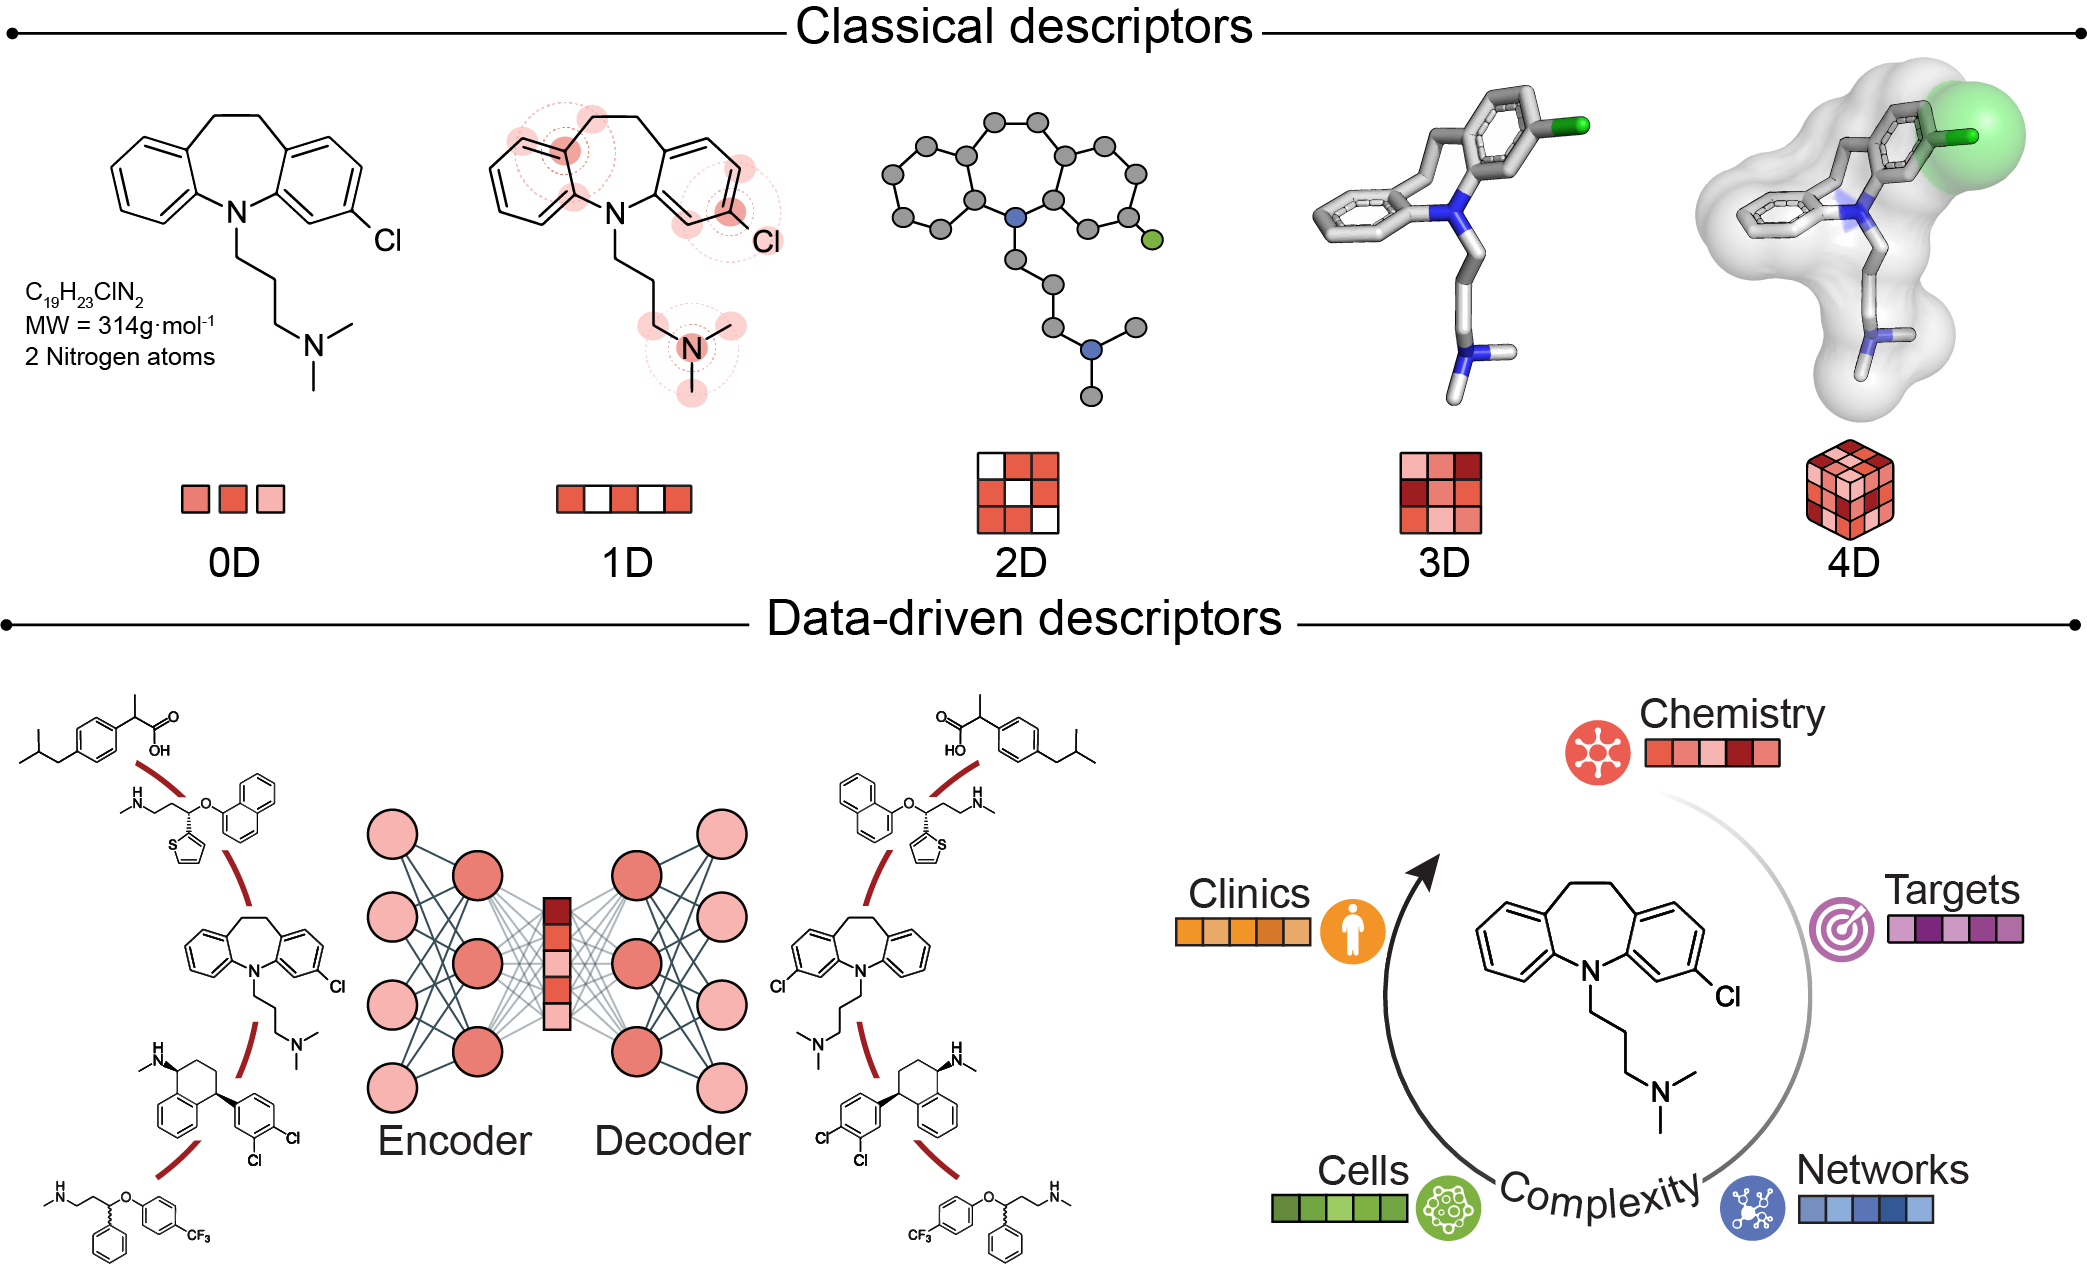
\includegraphics[width=\linewidth]{figures/Introduction/figure1_COCB.png}
  \caption{
    \textbf{Small molecule descriptors --encoding chemical molecules through their chemistry and bioactivity.} 
     \hl{Classical small molecule descriptors may include global molecular properties (0D, e.g. molecular weight), the presence of specific structural features (1D, e.g. ECFPs), molecular topology (2D, e.g. graphs), molecular conformation (3D, e.g. atom cartesian coordinates) or environment-dependent properties (4D, e.g. interactions with the protein target). Data-driven descriptors may be purely chemical, usually through the use of autoencoders, or encapsulating bioactivity information such as protein binding, induced gene expression changes or clinical outcomes.} 
    \rule[0ex]{\textwidth}{0.5pt}
  }
  \label{Introduction_Fig2}
\end{figure}

In practice, representing chemical compounds in a meaningful way for cheminformatics-related tasks requires the selection of a small molecule numerical descriptor. Molecular descriptors allow for the mathematical treatment of chemical and structural features of molecules and facilitate their subsequent use in computational applications. 


Various strategies exist to generate such descriptors (Fig \ref{Introduction_Fig2}). The simplest approaches account for global molecular properties (0D, e.g. molecular weight) or the presence of particular structural features (1D). Of particular interest are the broadly used extended-connectivity fingerprints (ECFPs \cite{rogers_extended-connectivity_2010}, encoding the circular environment of each atom up to a specific radius) and the molecular access system keys (MACCS Keys \cite{durant_reoptimization_2002}, accounting for the presence or absence of a specific set of pre-defined chemical groups), both being 1D small molecule fingerprints. Additionally, the molecular topology (2D, e.g. distance matrices between atoms) or the spatial information of the atoms (3D, e.g. cartesian coordinates) can be encapsulated by conveniently representing molecules as chemical graphs (atoms being nodes and bonds being edges) \cite{devinyak_3d-morse_2014}. Finally, further sophisticated methods capture environment-dependent properties, such as functional regions or intramolecular interactions (4D, e.g. energetically favorable binding sites or multiple MD-derived conformational states)\cite{pastor_grid-independent_2000, riniker_molecular_2017}. Although representing compounds with relatively complex frameworks (i.e. graphs) may provide a more natural depiction of molecules, simple 1D fingerprints offer numerous advantages, particularly in terms of computational efficiency, search speed, simplicity and interpretability \cite{rogers_extended-connectivity_2010}. In summary, these chemical descriptors are at the core of chemoinformatics and are still the first choice in most applications\cite{david_molecular_2020, cereto-massague_molecular_2015}.

However, the last years have witnessed the expansion of a new generation of molecular descriptors. Such descriptors, deemed to be data-driven and based on deep learning approaches, are engineered on the basis of large-scale chemistry databases and are thus adaptable to a given task or region of the chemical space of small molecules\cite{sanchez-lengeling_inverse_2018}. In particular, graph and text-based autoencoders\cite{hinton_reducing_2006, baldi_autoencoders_2012} are able to embed the information provided by 2D molecule structures and SMILES strings, respectively, into a dense numerical vector belonging to a “latent space” \cite{jin_hierarchical_2019, gomez-bombarelli_automatic_2018, liu_constrained_2018, polykovskiy_molecular_2020}. Simple measures such as Euclidean distances within the latent space are able to capture chemical similarity and, when coupled to machine learning algorithms, these descriptors have shown state of-the-art performance in several biophysics and physiological benchmark datasets\cite{wu_moleculenet_2018}.

\subsection{Extending the similarity principle beyond chemical structures}
\label{Introduction_extending}

A natural extension of the first generation of data-driven chemical descriptors is to include the wealth of bioactivity information available in the databases, to encapsulate, in the form of bioactivity descriptors, the experimental evidence gathered over years of research. Indeed, the use of bioactivity signatures enable the exploration of the drug-like chemical space in a biologically relevant manner. 

In pioneering work, instead of focusing on chemical structures, Kauvar et al. \cite{kauvar_predicting_1995} characterized a set of compounds according to their ability to bind a panel of 18 receptors and used these affinity profiles to assess similarities between them. The idea of relating small molecules based on their target profiles was further developed over the next years\cite{paolini_global_2006, keiser_predicting_2009}, enhancing the performance in classical chemoinformatics tasks (e.g. target prediction). In a more complex attempt to capture phenotypic effects induced by drug activity in cells, MacDonald et al. \cite{macdonald_identifying_2006} used a protein complementation assay to monitor the status of several cellular pathways after compound perturbation. Then, they derived pathway activity fingerprints for over a hundred compounds and found that pathway-based similarities strongly correlated with known structure-activity relationships. Similarly, Young et al. \cite{young_integrating_2008} combined automated microscopy with image analysis to profile the biological effects of a compound library. They integrated the resulting phenotypic profiles with the chemical structure of the compounds and their predicted targets and found that the combination of the three features had a substantially higher capacity to identify mechanisms of action than either one of them alone.

Indeed, the popularity of HTS assays has revealed that it is possible to establish relationships between compounds based on their functional activity rather than their chemical structure. For instance, it was suggested that molecules triggering similar transcriptional responses in cell lines might share mechanisms of action, an observation that inspired the implementation of the connectivity map \cite{lamb_connectivity_2006} and the following library of integrated network-based cellular signatures (LINCS L1000) \cite{subramanian_next_2017} initiatives. These libraries provide a catalog of transcriptional signatures in different cell lines, measured as a result of a systematic screening of genetic (CRISPR or shRNA) and pharmacological perturbations, which has been exploited, for instance, to suggest potential targets for a given compound\cite{sawada_predicting_2018}. Likewise, molecules that inhibit the growth of a similar subset of cell lines (i.e. that have similar sensitivity profiles) \cite{holbeck_analysis_2010} or drugs that elicit similar side effects, also tend to share mechanisms of action \cite{campillos_drug_2008}, even if their chemical structures appear to be unrelated.

Building upon these seminal works, our lab recently presented the Chemical Checker (CC), a resource that integrates the major chemogenomics and drug activity repositories and represents the largest collection of small molecule bioactivity signatures available to date \cite{duran-frigola_extending_2020}. The CC gathers experimentally determined bioactivity data for about 1M small molecules in the medicinal chemistry space and provides bioactivity descriptors in five levels of increasing biological complexity. The first level of descriptors characterizes the chemical properties of the compounds, including their 2D and 3D structures, scaffolds, functional groups, and physicochemical properties. The second level captures information on the protein receptors of the molecules, including known mechanisms of action, metabolizing enzymes and HTS binding assays. Descriptors in the third level of complexity address the propagation of the target perturbations triggered by the small molecules, including protein-protein interactions and pathways provided by several types of biological networks. The fourth level of signatures captures the bioactivity of the compounds measured at the cellular level, with assays including differential gene expression and sensitivity profiles in cancer cell-line panels. Finally, for the few compounds that reached clinical stages, the fifth level of CC signatures encodes details on their therapeutic areas, adverse side effects and drug-drug interactions.

A known limitation of the CC is that the number of molecules with reported bioactivities diminished at each level of complexity, and thus, we could only derive a limited set of bioactivity descriptors corresponding to a minority of well-characterized compounds. To extend the coverage of bioactivity descriptors to uncharacterized molecules, we trained a collection of deep neural networks (i.e. ‘signaturizers’) that are able to infer bioactivity signatures for any compound of interest, even when only its chemical structure is available. We were able to assign a confidence score to the predictions of the signaturizers and systematically apply them to sets of compounds beyond drug molecules, including plant metabolites and food ingredients\cite{bertoni_bioactivity_2021}.

Overall, bioactivity signatures provide a complementary means to describe small molecules, focusing on the integration of multiple types of experimental data \cite{wassermann_opportunities_2015}. Indeed, these descriptors have proven useful to navigate the chemical space in a biologically relevant manner and boost the performance in many drug discovery tasks that typically rely on chemical descriptors, such as target identification and toxicity prediction\cite{bertoni_bioactivity_2021}.

\subsection{Bioactivity in three dimensions}
\label{Introduction_bioactivity}

In the quest to leverage experimental data for generating bioactivity descriptors, chemical compounds represent only one part of the equation. These compounds (e.g. drugs) must physically interact with the disease-related target (e.g. a protein) to modulate its activity and exert the corresponding therapeutic effect, as assumed under the reverse pharmacology paradigm\cite{takenaka_classical_2001, hacker_pharmacology_2009}. Protein-ligand physicochemical interactions are three-dimensional, fully dependent on the chemical and structural complementarity between both entities\cite{kitchen_docking_2004, mcgovern_specific_2003}. 

Stereoisomerism refers to the type of isomerism where chemical compounds have identical molecular formulas and atom connectivities but differ in the three-dimensional spatial arrangement of their atoms \cite{gold_iupac_2019}. Since biological matter is intrinsically chiral (i.e. distinguishable from its mirror image), stereoisomeric small molecules may be differently absorbed, distributed, metabolized and excreted (i.e. pharmacokinetics) as well as exhibit completely distinct bioactivity profiles (and thus therapeutic effects, i.e. pharmacodynamics) \cite{inaki_cell_2016, mcconathy_stereochemistry_2003}. While pharmacological differences between stereoisomers are commonly expected in the case of diastereomers (stereoisomers that are not mirror images and exhibit distinct chemical properties, e.g. cisplatin and transplatin \cite{dasari_cisplatin_2014, trudu_coordination_2015}), such differences may not be as apparent in the case of enantiomers. Indeed, enantiomers are non-superimposable mirror images of each other whose separation and purification are usually challenging due to their identical physicochemical properties in non-chiral environments\cite{ward_chiral_2012}. An illustrative example is the case of (S)-Penicillamine, an antiarthritic drug administered as an enantiomerically pure compound due to the high toxicity of (R)-Penicillamine, its enantiomeric counterpart\cite{aronson_meylers_2010}. 

The CC offers an unprecedented opportunity to explore large scale bioactivity data in the context of stereoisomerism, quantifying to which extent stereoisomer pairs exhibit distinct bioactivities (e.g. protein binding profiles). In addition, and although the relevance of stereoisomerism in pharmacological applications is well known, the enumeration of all possible stereoisomers given a parent compound is usually missed when creating large chemical libraries in favor of maximizing chemical diversity (i.e. covering a broad area of the chemical space)\cite{ruddigkeit_enumeration_2012}. In line with this, original signaturizers to infer bioactivity signatures for uncharacterized compounds are built on 2D molecular representations (ECFPs) and are thus unable to capture differences between stereoisomer pairs (i.e. the inferred signatures are identical). There is therefore a clear need to bridge the gap between small molecule three-dimensional conformations and bioactivity signatures by developing a new generation of stereochemically-aware signaturizers.

\subsection{Protein structures}
\label{Introduction_proteinstructures}






\renewcommand{\thesubsection}{\thechapter.\arabic{section}.\arabic{subsection}}
